
%\begin{wrapfigure}{r}{0.25\textwidth} %this figure will be at the right
%    \centering
%    \includegraphics[width=0.25\textwidth]{03_Dinamika_materijalne_tocke/zadatak_D702.png}
%\end{wrapfigure}

\noindent 
\textbf{\stepcounter{zadatak}
\thecjelina.\thezadatak.}
Na slici  je sustav od dva utega mase $m_1=6\ kg$ i $m_2=3\ kg$. koji su povezani tankom nerastezljivom niti. Nagib kosine na kojoj se nalazi uteg mase $m_1$ je $\alpha=35^\circ$, koeficijent kinetičkog trenja između kosine i utega iznosi $\mu_k=0,3$, a trenje na koloturi se zanemaruje. Koliki je iznos sile napetosti niti?
\begin{figure}[ht]%{r}{0.7\textwidth} % Inline image example
  \begin{center}
    \includegraphics[scale=0.30]{../03_Dinamika_materijalne_tocke/Zadatak_D702.png}
  \end{center}
  %\caption{Fish}
\end{figure}

